\section{Teórico}

  \definicion{Topic:} Advanced functionals: higher accuracy (hybrids), strongly correlated materials (DFT+U), weakly bound systems (van der Waals).

  \definicion{Speaker:} Stefano DE GIRONCOLI (SISSA, Italy).

\subsection{Funcionales en DFT: término XC}

  Existen diferencias generaciones o grupos de funcionales que van creciendo en precisión, pero esto conlleva un incremento en su complejidad (Fig. \ref{fig:jacob}): incluso el funcional más sencillo contiene información acerca de la densidad de carga del sistema.

  \begin{figure}[H]
      \centering
      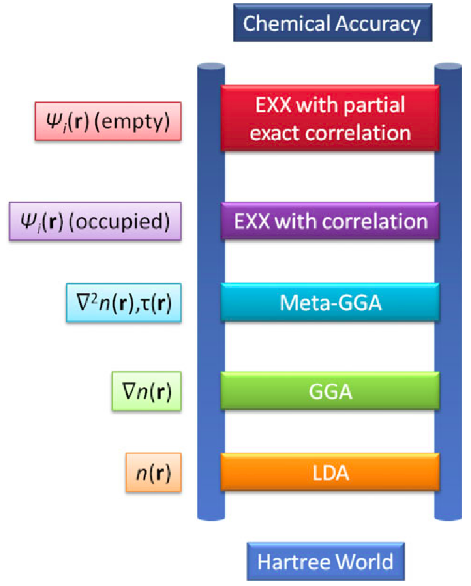
\includegraphics[scale = 0.5]{figs/D4/Jacob.png}
      \caption{Escalera de Jacob de las aproximaciones de DFT.}
      \label{fig:jacob}
  \end{figure}

  Los teoremas de Hohenberg-Kohn (HK) están relacionados a cualquier sistema que consista de electrones moviéndose bajo la influencia de un potencial externo:
    \begin{enumerate}
      \item \textbf{Primer teorema HK:} el potencial externo y, en consecuencia, la energía total son un funcional único de la densidad electrónica. Luego, la densidad electrónica del estado fundamental describe de manera unívoca el potencial y, por lo tanto, todas las propiedades del sistema, incluyendo la función de onda many-body. Se sigue que el espectro del Hamiltoniano también es un funcional único de dicha densidad basal. Particularmente, el funcional HK es una función universal de la densidad electrónica, no dependiendo de manera explícita del potencial externo.
        $$F[n] = T[n] + U[n]$$
      \item \textbf{Segundo teorema HK:} El funcional permite determinar la energía del estado fundamental si y sólo si la densidad electrónica es la del estado fundamental.
        $$F [n] = \underbrace{min}_{\Psi \rightarrow n} \bra{\Psi} T_e + W_{ee} \ket{\Psi}$$
    \end{enumerate}

  Se tiene entonces que para cualquier natural $N$ y potencial externo $v_{ext} (\vec{r})$ existe un funcional de desidad $F[n]$ tal que
    $$E [n] = F[n] + \int v_{ext} (\vec{r}) n (\vec{r}) d\vec{r}$$

  Partiendo de esta idea, KS plantean la energía cinética de un sistema ficticio de electrones no interactuantes.
    $$T_s[n] = \underbrace{min}_{\Psi \rightarrow n} \bra{\Psi} T_e\ket{\Psi}$$

  Con esta información se reescribe la ecuación de HK según del sistema interactuante según
    $$F[n] = T_s[n] + E_{Har} [n] + E_{XC} [n]$$

  Así la energía del sistema será
    $$E [n] = T_s[n] + E_{Har} [n] + E_{XC} [n] + \int v_{ext} (\vec{r}) n (\vec{r}) d\vec{r}$$

  Todo lo que quedó fuera al recurrir a este sistema no interactuante está contenido en el término XC. Este término es pequeño relativo a los demás términos que contribuyen a la energía total del sistema. Por este motivo es que incluso la aproximación más sencilla sigue siendo útil para los cálculos.

\subsection{L(S)DA}

  La aproximación más sencilla es Local (Spin) Density Approximation (L(S)DA), donde la "S" se pone según se esté considerando o no la contribución de spin. En este caso basta con conocer la densidad electrónica en cada punto del espacio.
    $$E_{XC} = E_{XC} [n]$$

  Asume que la densidad varía lentamente, tratando entonces a la densidad local como un gas homogéneo de electrones: el valor de la energía XC en una posición $\vec{r}$ se determina exclusivamente a partir del valor de la densidad en esa posición, \emph{i.e} el valor local de $n$.

  A pesar de su sencillez, ofrece resultados bastante razonables para el estado fundamental. Describe una gran variedad de propiedades para un amplio abanico de materailes: energía, estabilidad de fases, defectos termodinámicos, geometrías de equilibrio, funciones respuesta, etcétera. Si, además, consideramos la aproximación adiabática, la dinámica de la red es una propiedad del estado fundamental: puedo determinar propiedades vibracionales, termidonámicas y defectos. En general se observan buenas tendencias respecto a los valores experimentales. También da buenas tendencias.

  Las primeras limitantes son que da lugar a enlaces más cortos y más fuertes, dando en consecuencia módulos de Young mayores. Además los bandgaps son muy chicos.

  \Obs{Cuánto mayor sea tasa de cambio de la densidad, menos confiables son los resultados cuando se usa LDA.}

\subsection{GGA}

  Esta familia de funcionales conocido como Generalized Gradient Approximation (GGA) requiere información del gradiente local de la densidad electrónica además de la propia densidad electrónica.
    $$E_{XC} = E_{XC} [n, \nabla n]$$

  En realidad se utiliza el gradiente reducido, dado por
    $$\frac{\nabla n}{n^{\sfrac{4}{3}}}$$

  La densidad decae exponencialmente, por lo que denominador provoca que este cociente sea divergente para $r$ grande. Esto hace que en la región de mayor probabilidad de encontrar electrones (en torno al núcleo), el gradiente sea pequeño y acotado. Sin embargo, al alejarnos del núcleo la densidad cae y el gradiente reducido diverge. Se tiene entonces que el funcional puede considerar dos regiones: una más externa o superficial y una más interna o cercana al núcleo. Esto permite una mucho mejor descripción del sistema.

  El primero de este tipo fue PW91 (Perdew-Wang). Basándose en éste, simplificando las ideas, pero haciéndolas a su vez más potentes en sus resultados, surgió uno de los más usados: PBE (Perdew-Burke-Ernzerhof).

  Estos resuelven el overbinding del LDA. Se acercan al valor real, pero siguen estando por encima en algunos casos. Aunque sus efectos en los parámetros de red son más aleatorios. De todas formas logra describir mucho mejor las estructuras cristalinas de los elementos. Además, GGA es importante para sistemas magnéticos, particularmente para el hierro: LDA dice que es no magnético, pero GGA logra describir que tiene propiedades magnéticas.

  Los problemas que había con LDA y que GGA no logra superar son:
    \begin{itemize}
      \item Buenas tendencias para enlaces fuertes (covalente, iónico, metálico), pero no para pequeñas superposiciones.
      \item Las autoitneracciones no son 100 \% canceladas. Cuanto más localización, la autointeracción se vuelve más relevante. También en sistemas sólidos que conservan mucho sus cualidades atómicas (orbitaes moleculares con apariencia de orbitales atómicos).
      \item Como son tan locales, no logran ver cosas no localizadas como las vdW. Cuando se llega a un resutlado acorde suele ser más por errores numéricos.
    \end{itemize}

\subsection{Solución a la autointeracción}

  Para resolver el problema de las autointeracciones se recurre a SIC (Self Interaction Correction), DFT+U o funcionales híbridos.

  En principio, en DFT los electrones interactúan con un potencial efectivo generado por todos los electrones, incluido él mismo. Cuando la densidad es más dispersa, el error de autointeracción es pequeño. Sin embargo, cuanto más localizado se vuelve, mayor es error. El problema también se presenta cuando cambia la localidad del orbital, por ejemplo en una redox que transfieren un electron desde un estado deslocalizado a uno localizado. Esto es usual en óxidos de metales de transición, generando errores del orden de los eV.

  El problema de la autointeracción viene de la mano del tratamiento que se le hace a la aproximación de XC en términos de electrostática: LDA es bueno describiendo el movimiento de un electrón en un potencial medio, resultando mejor cuanto más lejos estén los electrones entre sí.

  El funcional SIC no es muy utilizado, pero su desarrollo fue conceptualmente importante. Es una solución ad hoc orbital-dependent, pero complicada.

  Los funcionales híbridos combinan SIC con LDA/GGA. Es muy caro de aplicar con una base de ondas planas. DFT+U son funcionales útiles para describir materiales fuertemente correlacionados. Recientemente ha sido aplicado a materiales más generales con resultados prometedores.

\subsection{Conexión adiabática}

  Dijimos que HK considera un Hamiltoniano con todas las interacciones \emph{prendidas} mientras que KS describe un sistema no interactuante. Podemos pensar que ambos funcionales son dos casos extremos de una misma situación. La conexión la podemos hacer introduciendo un parámetro $\lambda \in[0,1]$ KS (0) hasta el sistema many-body de HK (1). El parámetro varía de forma continua y adiabática.

  Utilizando el teorema de Hellmann-Feynman, se llega a que la suma entre la energía de Hartree y la XC es el promedio desde la no interacción hasta interaccion full sobre el valor de expectación de la matriz de interacción.

  Becke asume que la variacion de la perturbación con $\lambda$ cambia suave y linealmente. Para $\lambda=0$ es el XC de Hartree computado con los orbitales KS, mientras que para $\lambda=1$ se requieren otras aproximaciones como LDA. Esto es lo que se conoce como el funcional half-half (HH). De acá se pueden ver B3LYP, PBEO y HSE.

\subsection{Energía de Hartree-Fock}

  El término HF es muy caro de calcular (10 a 100 veces más) con PW ya que va y vuelve entre espacios duales y en cada uno hace cálculos caros para cada orbital.

  Cuando escribimos la integral HF en forma recíproca, tiene una divergencia en $q+G=0$. Este no es un problema porque es una singularidad evitable, pero de manera no trivial: remueven el término divergente y luego agregan un término que contiene esta divergencia atenuada con una exponencial.

\subsection{DFT+U}

  La idea de hacer DFT+U es tratar la fuerte interacción Coulómbica de los electrones localizados (la cual no está bien desripta con LDA ni GGA) agregando un término Hubbard. Esto es relevante principalmente en metales donde las interacciones Coulómbicas son particularmente fuertes en los orbitales d y f.
   $$E_{DFT+U} = E_{DFT} + E_{U} \Rightarrow E_{U} = \frac{U}{2} \sum_a tr\left[ \rho_a (1 - \rho_a)  \right]$$

  donde $\rho_a$ es la matriz de ocupación de OA. En otros términos estamos agregando una penalización a la energía DFT para forzar la matriz de ocupación a alcanzar la idempotencia (o completamente ocupada o compeltamente desocupada). Las ocupaciones fraccionarias no son compatibles con valores altos de U: a mayor U, mayor penalty.

  \Obs{Para tener una idea gráfica, podemos mapear una parábola invertida donde $U$ es su máximo: pushea al sistema a caer en ocuáncias 0 ó 1 ya que las fracciones tienen un precio, siendo el $U$ el más caro cuando la ocupación es $\sfrac{1}{2}$. El término de Hubbard implica agregar un potencial de Hubbard a la ecuacion KS.}

  Calcular $U$ en sólidos no es tan sencillo ya que uno no tiene tanto control sobre cuántos electrones se disponen en cada obrital: esto lo decide KS. Así que hay que sacarlo de la curvatura de $E_{DFT}$ con respecto al número de ocupación. En la práctica se introducen perturbaciones locales sobre grandes superceldas y luego se calculan las variaciones en la energía con respecto a los números de ocupación. Al invertir la función respuesta, sale $U$.



\subsection{Funcionales de vdW}

  Se trata de un efecto de correlación no local incluido en XC, pero que no está considerado en ningún funcional: vdW necesita considerar al menos 2 puntos.

  Hay varias opciones:
    \begin{itemize}
      \item Despreciarlo.
      \item Agregar una correción de dispersión amortigüada empírica (Grimme).
      \item Desarrollar un funcional XC no local.
    \end{itemize}

\subsection{Aspectos generales}

  \begin{itemize}
    \item \textbf{L(S)DA:} simples y bien definidos. Dan una buena geometría, pero overbinding.
    \item \textbf{GGA:} gran variedad para elegir, con mejoras en los resultados de energía. Buena geometría.
    \item \textbf{Meta-GGA:} muy complicados y no tan usados.
    \item \textbf{SIC, DFT+U, Híbridos:} atacan el problema de la autointeracción.
    \item \textbf{vdW:} falta mucho.
  \end{itemize}

\section{Q\&A}



\section{Hands-on}

\definicion{Topic:} Functionals.

\definicion{Speaker:} Iurii TIMROV (EPFL, Switzerland).

\subsection{}

\subsubsection{Objetivo}

\subsubsection{Pasos}

\subsubsection{Resultados}



--------------------------------------------------------------------------------

EJEMPLO DEL HIERRO (1)

  Para determinar sobre qué orbitales debemos apicar la corrección, debemos recurrir a una parte de código duro de QE (aún no implementado vía input): $set\_hubbard\_n.f90$ y $set\_hubbard\_l.f90$ donde $n$ y $l$ refiere respectivamente a los números cuánticos principal y orbital.

  Queremos aplicar la $U$ sobre los electrones 3d ($n=3$ y $l=2$).

  Quiero hacer DFT+U: $lda\_plus\_u = .true.$.

  Versiones de DFT+U: $lda\_plus\_u\_kind = 0,1,2$. Tenemos que $0$ es la versión más simple, $1$ es más completa y $2$ es DFT+U+V.

  $U\_projection\_type = 'atomic'$ Le dice qué tipo de funciones considerar para la matriz de ocupación. En este caso son funciones tipo atómicas. Podría ser $'orto'$ y serían atómicas, pero mútuamente ortogonales, incluyendo también los oxígenos. Esto arroja resultados más precisos.

  $Hubbard\_U(i) = 1.d-8$ donde $i$ es el índice del átomo sobre el cual aplicar la corrección. Son casi cero para hacer un cálculo PBESol (PBE sobre sólidos), pero no cero para activar la maquinaria DFT+U. Esto generará información extra en el output que nos va a servir (LDA+U parameters al final: spin 1 = up y spin 2 = down). Igual no vamos a hacer ninguna correción U, sólo cheateamos al código (alto jáker). Como son hierros cistalográficamente equivalentes, deben tener el mismo valor.

  https://www.materialscloud.org/work/tools/qeinputgenerator

  La nscf es para tener la PDOS. Con $nbnd = 35$ agrega más antiestados para que la cosa salga linda.

  Primer átomo: spin 1 prácticamente leno, pero spin 2 ocupaciones parciales (0.2). En el segundo hierro tenemos las cosas invertidas. Ver cómo esto se refleja en la PDOS: la majority está toda por debajo de la Fermi y para la minority tenemos un poco abajo y otro poco arriba de la energía de Fermi. Tenemos que DFT dice que el sistema es metálico.

  Cuando hacemos la corrección Hubbard ahora tenemos que el sistema es un aislante ya que se nos presenta el bandgap, lo cual es experimentalmente correcto.

  ¿Cómo elegir U?  Hay un ejecutable: hp.x (Hubbard Parameters). Tiene un input super cortito y al pie. No es conveniente para close-shell systems. De ahí saca el 4.6 eV.

  DFT-U-V: fomulación extendida que considera una interacción de Hubbard entre sitios interatómicos. La contribución U depende de un sitio, mientras que la contribución V depende de sitios. Ambos se pueden calcular con hp.x. Este funcional extendido tiene más flexibilidad: no sólo arregle el problema de localización, sino que también corrije la interacción con ligandos.

  \begin{figure}[H]
      \centering
      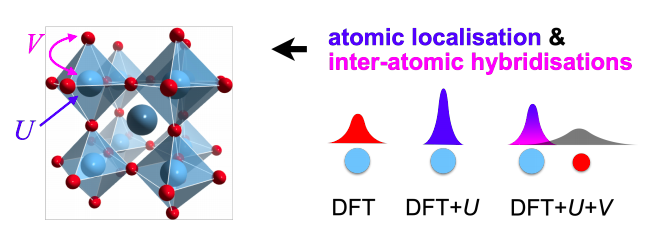
\includegraphics[scale = 0.6]{figs/D4/DFT+U+V.png}
      \caption{DFT+U+V.}
      \label{fig:DFT+U+V}
  \end{figure}

  \Obs{DFT+U suele ser peor que los funcionales híbridos.}

  --------------------------------------------------------------------------------

  EJEMPLO DEL SILICIO (2)

  Los funcionales híbridos son realmente caros. $input\_dft$ le decimos decimos qué funcional híbrido usar (pbe0, b3lyp, hse). Tomar un PP que sea lo más cercano a lo híbrido que queremos. Le damos la mesh de puntos. Si queremos que se encargue de la singularidad usamos $x\_gamma\_extrapolation = .true.$. Le pedimos que la integre analíticamente diciendo $exxdive\_treatment = 'gygi-baldereschi'$.

  Usar extrapolación permite usar una $k$-mesh más chiquita.

  --------------------------------------------------------------------------------

  EJEMPLO DEL Grafito (3)

  Interacción de vdW entre layers de grafeno. La distancia de equilibrio entre layers es muy pequeña con LDA y muy larga con GGA. Esto indica que debems considerar vdW.

  Tratar de hacer los 7 cálculos de las filminas (vc-relax). Algunos no locales, otros semiempírico. Finalmente usar LDA y GGA.

  $input\_dft$ cambia el funcional (cambia desde el comienzo la movida tropical).
  $vdw\_corr$ correcciones que se hace al final del cálculo (tipo PP).
